\chapter{Выбор компонентов}

По результатам расчетов были выбраны:
\begin{enumerate}
\item резисторы MO-200 (С2-23) CF-100 (С1-4) ёмкостью 200 Ом;
\item конденсатор К10-17Б ёмкостью 2,2 мкФ;
\item конденсатор К10-17Б ёмкостью 1 мкФ. 
\end{enumerate}

\begin{figure}[h!]
	\centering
	\caption{Параметры операционного усилителя }
	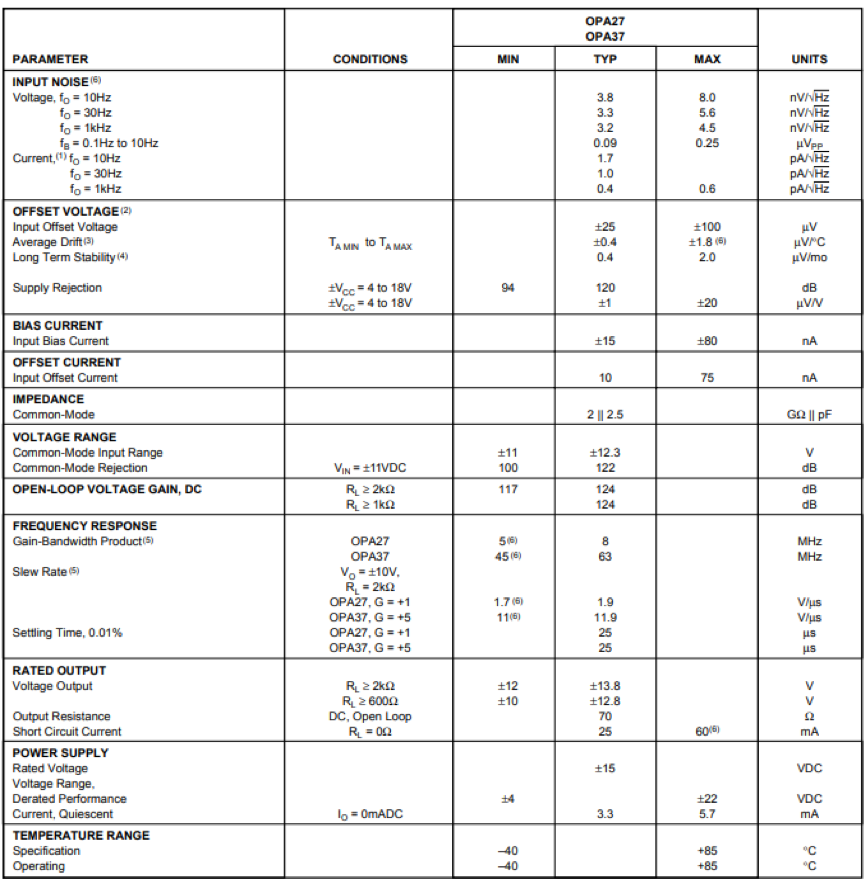
\includegraphics{images/1.png}
\end{figure}

\begin{figure}[h!]
	\centering
	\caption{Параметры конденсатора К10-17Б (1 мкФ)}
	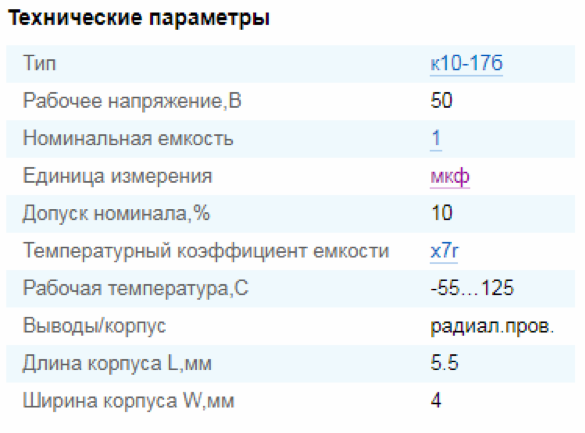
\includegraphics{images/2.png}
\end{figure}

\begin{figure}[h!]
	\centering
	\caption{Параметры конденсатора К10-17Б (2,2 мкФ)}
	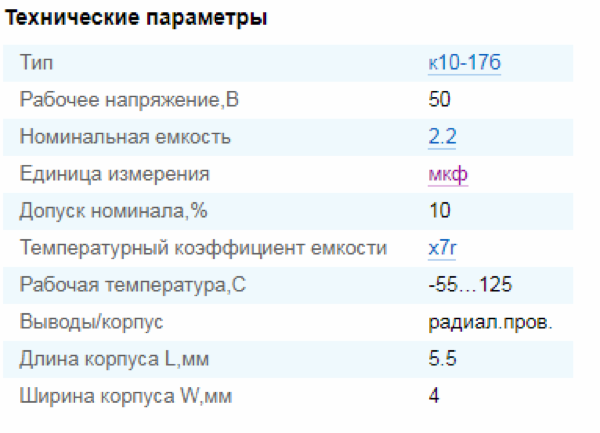
\includegraphics{images/3.png}
\end{figure}

\begin{figure}[h!]
	\centering
	\caption{Параметры резистора MO-200 (С2-23)}
	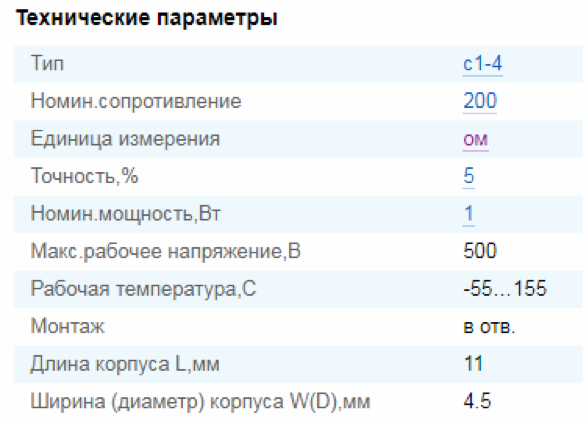
\includegraphics{images/4.png}
\end{figure}
